\documentclass[border=10pt]{standalone}
\usepackage{pgfplots}
\pgfplotsset{compat=1.18}
\usepgfplotslibrary{groupplots,fillbetween}
\begin{document}
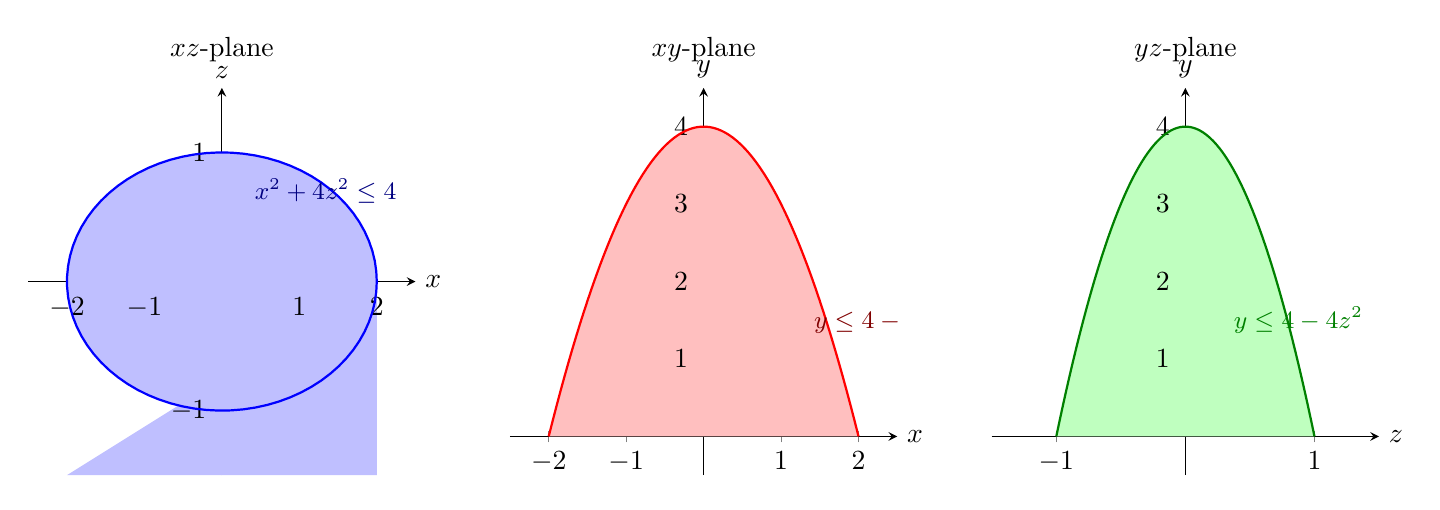
\begin{tikzpicture}
\begin{groupplot}[
    group style={group size=3 by 1, horizontal sep=1.2cm},
    width=6.5cm, height=6.5cm,
    axis lines=middle,
    every axis x label/.style={at={(ticklabel* cs:1)}, anchor=west},
    every axis y label/.style={at={(ticklabel* cs:1)}, anchor=south},
    xtick={-2,-1,1,2}, ytick={-1,1},
    enlargelimits=false,
]

% xz-plane: ellipse
\nextgroupplot[
    xlabel={$x$}, ylabel={$z$},
    title={$xz$-plane},
    xmin=-2.5, xmax=2.5, ymin=-1.5, ymax=1.5,
]
\addplot[name path=A, blue, thick, domain=0:2*pi, samples=80] ({2*cos(deg(x))}, {sin(deg(x))});
\addplot[name path=B, draw=none, domain=-2:2, samples=2] {-1.5};
\addplot[blue!25] fill between[of=A and B];
\node[blue!50!black, anchor=west] at (axis cs:0.3, 0.7) {\small $x^2 + 4z^2 \leq 4$};

% xy-plane: parabola y = 4 - x^2
\nextgroupplot[
    xlabel={$x$}, ylabel={$y$},
    title={$xy$-plane},
    xmin=-2.5, xmax=2.5, ymin=-0.5, ymax=4.5,
    ytick={1,2,3,4},
]
\addplot[name path=A, red, thick, domain=-2:2, samples=80] {4 - x^2};
\addplot[name path=B, draw=none, domain=-2:2, samples=2] {0};
\addplot[red!25] fill between[of=A and B];
\node[red!50!black, anchor=west] at (axis cs:1.3, 1.5) {\small $y \leq 4 - x^2$};

% yz-plane: parabola y = 4 - 4z^2
\nextgroupplot[
    xlabel={$z$}, ylabel={$y$},
    title={$yz$-plane},
    xmin=-1.5, xmax=1.5, ymin=-0.5, ymax=4.5,
    ytick={1,2,3,4},
]
\addplot[name path=A, green!50!black, thick, domain=-1:1, samples=80] {4 - 4*x^2};
\addplot[name path=B, draw=none, domain=-1:1, samples=2] {0};
\addplot[green!25] fill between[of=A and B];
\node[green!50!black, anchor=west] at (axis cs:0.3, 1.5) {\small $y \leq 4 - 4z^2$};

\end{groupplot}
\end{tikzpicture}
\end{document}